\section{ZnO Substrate Yields the Best Ag Thin Film}

\begingroup
\begin{figure}[ht]
  \centering
  \subfigure[]{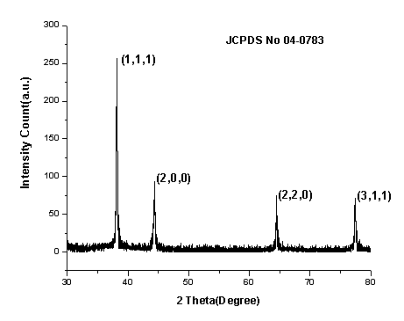
\includegraphics[width=0.49\linewidth]{Chap4/plots/Picture4a.pdf}}\label{Chap:Ag/ZnO:fig:4a}
  \subfigure[]{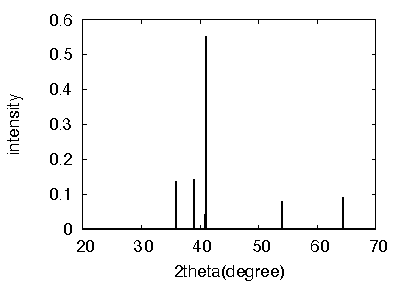
\includegraphics[width=0.49\linewidth]{Chap4/plots/Picture4b.pdf}}\label{Chap:Ag/ZnO:fig:4b}
\caption[Simulated XRD plots of FCC and HCP Ag]{Simulated XRD plots of FCC and HCP Ag. (a) Simulated XRD results for FCC Ag. (b) Simulated XRD results for HCP Ag.}
  \label{Chap:Ag/ZnO:fig4}
\end{figure}
\endgroup

In this section, we will answer the question that which substrate type is best for Ag thin film deposition. Three different bond lengths will be used: 3.3$\angstrom$, 2.9$\angstrom$, 2.3$\angstrom$. 3.3$\angstrom$ is equivalent to the ZnO lattice constant. 2.9$\angstrom$ is for Ag bond length, which means this substrate has a zero misfit for Ag thin film. At last, 2.3$\angstrom$ is selected for simulating a negative lattice mismatch factor, where lattice mismatch factor($f_{mismatch}$) is defined via:
\begin{align}
    f_{mismatch} = \frac{a_{substrate} - a_{film}}{a_{substrate}}
    \label{Chap:Ag/ZnO:eq:mismatch}
\end{align}
Where $a_{substrate}$ and $a_{film}$ are the lattice constant of substrate and thin film, respectively. And the bond strength is fitted to match the Ag adsorption energy on fully-saturated ZnO substrates as we mentioned in Section. \ref{sec:Hcoverage}.

\begingroup
\begin{figure}[!ht]
  \centering
  \subfigure[]{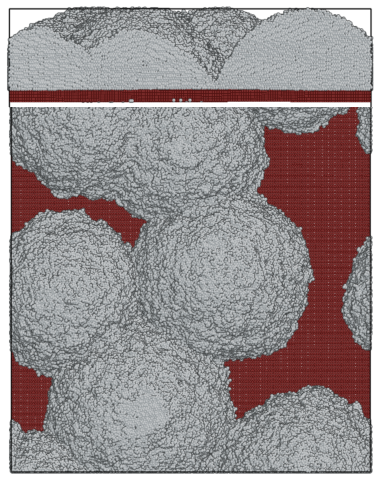
\includegraphics[width=0.4\linewidth]{Chap4/plots/Picture5a.pdf}}\label{Chap:Ag/ZnO:fig:5a}
  \subfigure[]{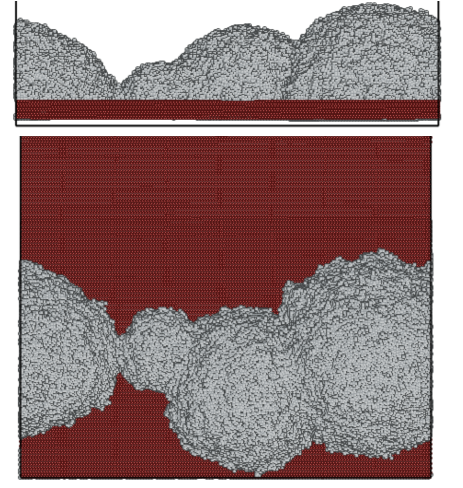
\includegraphics[width=0.4\linewidth]{Chap4/plots/Picture5b.pdf}}\label{Chap:Ag/ZnO:fig:5b}\\
  \subfigure[]{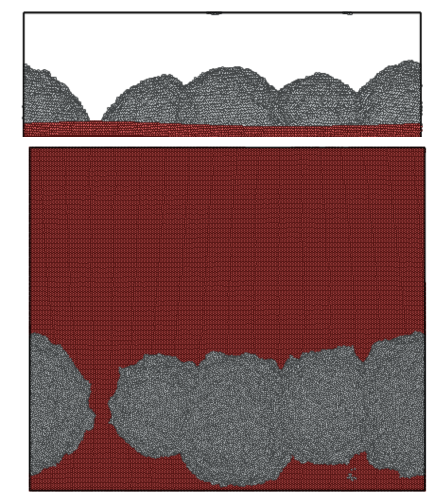
\includegraphics[width=0.45\linewidth]{Chap4/plots/Picture5c.pdf}}\label{Chap:Ag/ZnO:fig:5c}
\caption[GCMC simulated Ag thin film morphology on hexagonal substrates.]{GCMC simulated Ag thin film morphology on hexagonal substrates with bond length of (a) 2.3$\angstrom$, (b) 2.9$\angstrom$, and (c) 3.3$\angstrom$. Top sub-figures are side views of 40 \ac{ML} atoms and bottom sub-figures are top views.}
  \label{Chap:Ag/ZnO:fig5}
\end{figure}
\endgroup

In order to characterize the orientation of thin films, simulated \ac{XRD} will be evaluated. From experimental \ac{XRD} plot, Ag {111} orientation will have a strong peak around $38^{\circ}$ from JCPDS No 04-0783 \cite{AgPDF}. We also simulated \ac{XRD} results for \ac{HCP} Ag in order to characterize the crystalline quality of Ag thin films. And we can see if Ag is in \ac{HCP} structure, there will be strong peaks around $35.86^{\circ}$, $38.95^{\circ}$, and $40.96^{\circ}$.

\begingroup
\begin{figure}[!ht]
  \centering
  \subfigure[]{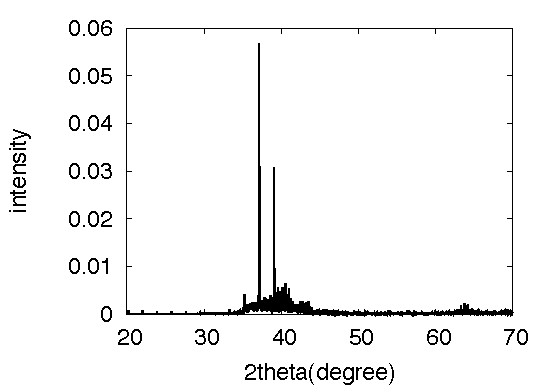
\includegraphics[width=0.49\linewidth]{Chap4/plots/Picture6a.pdf}}\label{Chap:Ag/ZnO:fig:6a}
  \subfigure[]{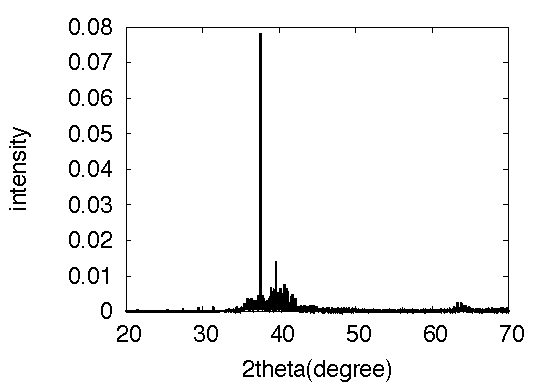
\includegraphics[width=0.49\linewidth]{Chap4/plots/Picture6b.pdf}}\label{Chap:Ag/ZnO:fig:6b}
  \\
  \subfigure[]{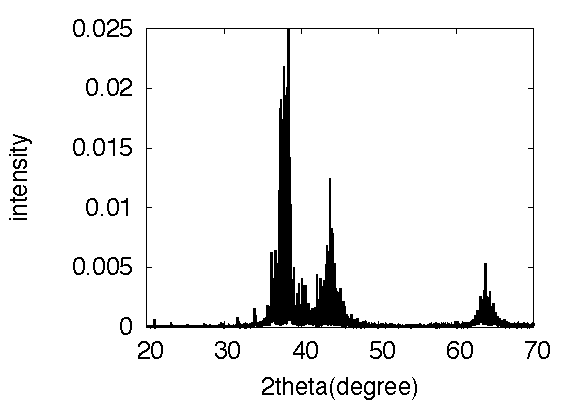
\includegraphics[width=0.49\linewidth]{Chap4/plots/Picture6c.pdf}}\label{Chap:Ag/ZnO:fig:6c}
\caption[Simulated XRD results of Ag thin film on hexagonal substrates.]{Simulated \ac{XRD} results of Ag thin film on hexagonal substrates with bond length of (a) 2.3$\angstrom$, (b) 2.9$\angstrom$, and (c) 3.3$\angstrom$. The substrate with 2.9$\angstrom$ bondlength (similar to Ag deposition on Ag (111) substrate) shows best Ag \{111\} orientation.}
  \label{Chap:Ag/ZnO:fig6}
\end{figure}
\endgroup

We first investigated the results of the hexagonal substrate with 3 different bond lengths, as shown in Fig. \ref{Chap:Ag/ZnO:fig5}. A 50$\angstrom$x50$\angstrom$ substrate is used for Ag deposition. Assuming Ag thin films all follow {111} orientation, there will be $\sim$ 50,000 Ag atoms/layer. We deposit 2,000,000 Ag atoms, which is equivalent to a 40 \ac{ML}s (10 nm thickness) of Ag atoms, then observed the morphology of thin films on different substrates. As shown in Fig. \ref{Chap:Ag/ZnO:fig5}, the left sub-figure is for 2.3$\angstrom$ bond length, the middle one for 2.9$\angstrom$, and the right one for 3.3$\angstrom$. Ag thin film follows an island-like growth pattern with all three lattice constants/bond lengths. Note that the middle one, with a bond length of 2.9$\angstrom$, which is similar to the situation of Ag on Ag(111) island growth pattern \cite{li2008exploration}. For ZnO lattice constant (3.3$\angstrom$), still, island-like growth was observed for 10 nm thickness. Possible reasons could be: 1) a Ag chemical potential corresponding to $\sim 1 Pa$ is used, and this could be orders higher in the industrial-level sputtering chamber; 2) the substrate in the simulation is the perfect crystal, which does not consider the polycrystalline and surface defects. Those defect sites can have stronger binding to Ag adsorbates, thus they may increase the chance of surface nucleation; 3) detailed surface diffusion kinetics are ignored during \ac{GCMC} simulations.

\begingroup
\begin{figure}[!ht]
  \centering
  \subfigure[]{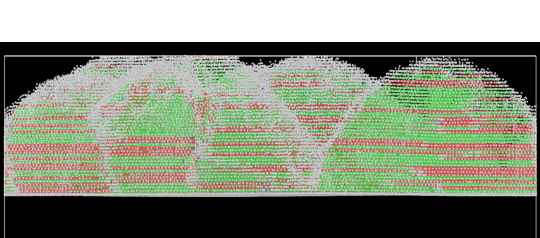
\includegraphics[width=0.75\linewidth]{Chap4/plots/Picture7a.pdf}}\label{Chap:Ag/ZnO:fig:7a}
  \\
  \subfigure[]{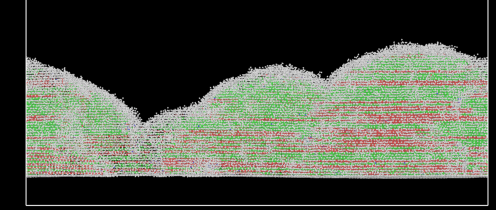
\includegraphics[width=0.75\linewidth]{Chap4/plots/Picture7b.pdf}}\label{Chap:Ag/ZnO:fig:7b}
  \\
  \subfigure[]{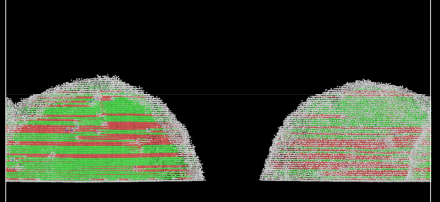
\includegraphics[width=0.75\linewidth]{Chap4/plots/Picture7c.pdf}}\label{Chap:Ag/ZnO:fig:7c}
\caption[Common neighbor analysis plots of Ag thin film on hexagonal substrates.]{\ac{CNA} plots of Ag thin film on hexagonal substrates with bond length of (a) 2.3$\angstrom$, (b) 2.9$\angstrom$, and (c) 3.3$\angstrom$. Green, red, and grey atoms indicate \ac{FCC}, \ac{HCP} structure and structure cannot be identified (Usually due to lack of neighboring atoms, e.g. surface or interface atoms, or amorphous-like atoms), respectively.}
\label{Chap:Ag/ZnO:fig7}
\end{figure}
\endgroup

\begingroup
\begin{figure}[!ht]
  \centering
  \subfigure[]{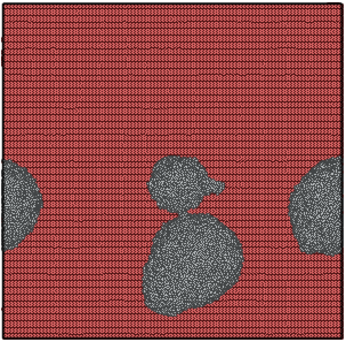
\includegraphics[width=0.3\linewidth]{Chap4/plots/Picture8a.pdf}}\label{Chap:Ag/ZnO:fig:8a}
  \subfigure[]{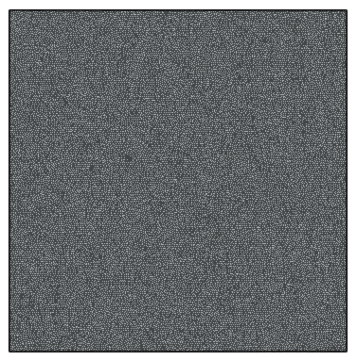
\includegraphics[width=0.3\linewidth]{Chap4/plots/Picture8b.pdf}}\label{Chap:Ag/ZnO:fig:8b}
  \\
  \subfigure[]{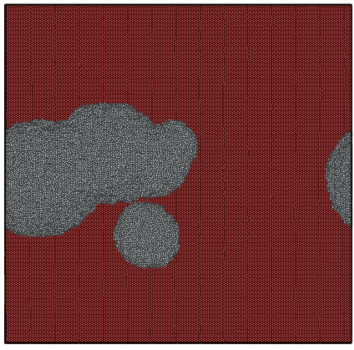
\includegraphics[width=0.3\linewidth]{Chap4/plots/Picture8c.pdf}}\label{Chap:Ag/ZnO:fig:8c}
  \subfigure[]{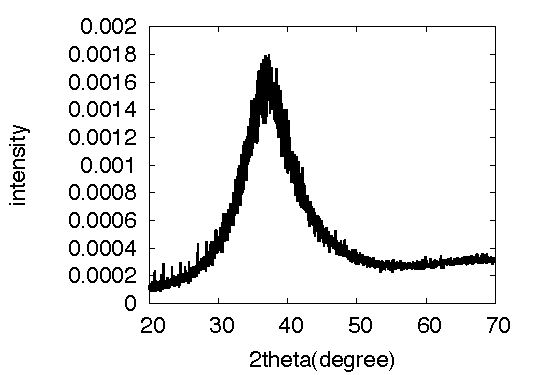
\includegraphics[width=0.49\linewidth]{Chap4/plots/Picture8d.pdf}}\label{Chap:Ag/ZnO:fig:8d}
  \\
  \subfigure[]{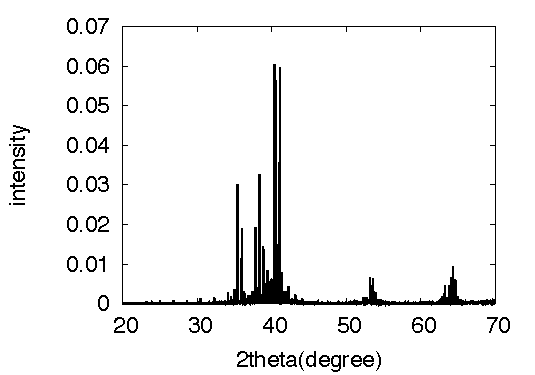
\includegraphics[width=0.49\linewidth]{Chap4/plots/Picture8e.pdf}}\label{Chap:Ag/ZnO:fig:8e}
  \subfigure[]{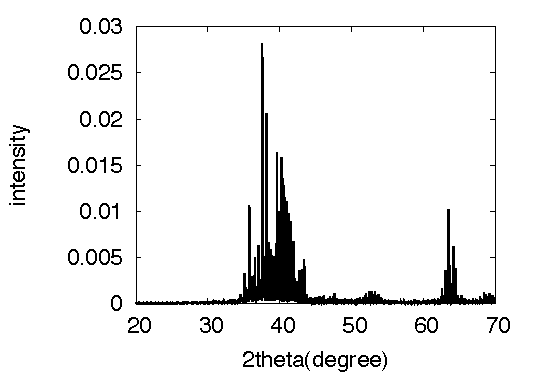
\includegraphics[width=0.49\linewidth]{Chap4/plots/Picture8f.pdf}}\label{Chap:Ag/ZnO:fig:8f}
\caption[GCMC simulation and simulated XRD results of Ag thin film morphology on rectangular substrates.]{Top-view of \ac{GCMC} simulated Ag thin film morphology on rectangular substrates with bond length of (a) 2.3$\angstrom$, (b) 2.9$\angstrom$, and (c) 3.3$\angstrom$. (d), (e), and (f) are corresponding simulated \ac{XRD} results of three Ag thin film  deposited on substrates with previously mentioned bond length.}
  \label{Chap:Ag/ZnO:fig8}
\end{figure}
\endgroup



Simulated \ac{XRD} results of hexagonal substrates are also plotted in Fig. \ref{Chap:Ag/ZnO:fig6}. The middle figure (similar to Ag deposition on Ag (111) substrate) shows best {111} orientation. For larger and smaller lattice constant, {111} orientation still persist but with broadened peaks and other peaks for {200} and {220}, as shown in Fig. \ref{Chap:Ag/ZnO:fig:6c}. Besides, \acf{CNA} \cite{kelton1991crystal} is also applied, to identify internal defects. All three lattice constant have similar amount of layered defects (like stacking faults or twin boundaries) as noted as \ac{HCP} layers in \ac{FCC} structures in Fig. \ref{Chap:Ag/ZnO:fig7}.

\begingroup
\begin{figure}[!ht]
  \centering
  \subfigure[]{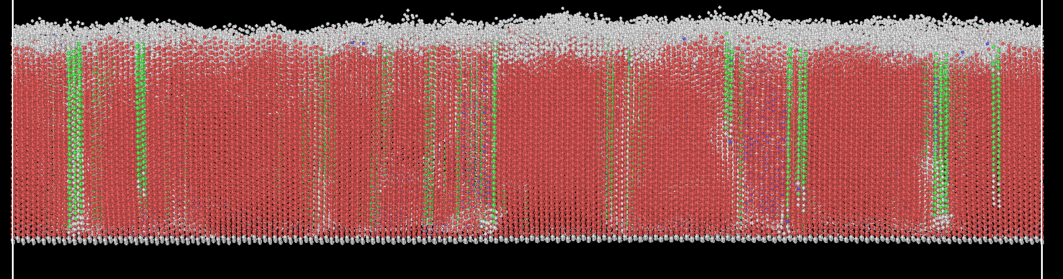
\includegraphics[width=0.99\linewidth]{Chap4/plots/Picture9a.pdf}}\label{Chap:Ag/ZnO:fig:9a}
  \\
  \subfigure[]{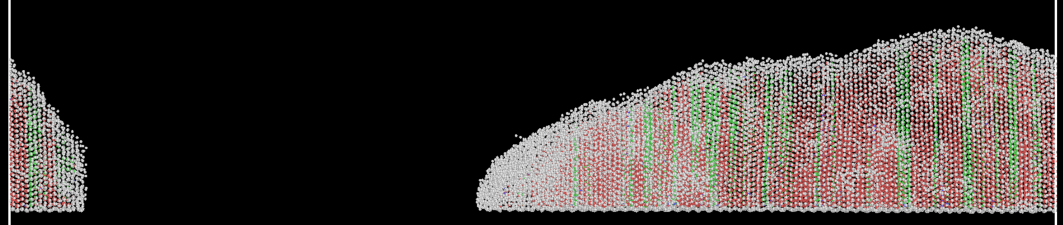
\includegraphics[width=0.99\linewidth]{Chap4/plots/Picture9b.pdf}}\label{Chap:Ag/ZnO:fig:9b}
  \\
  \subfigure[]{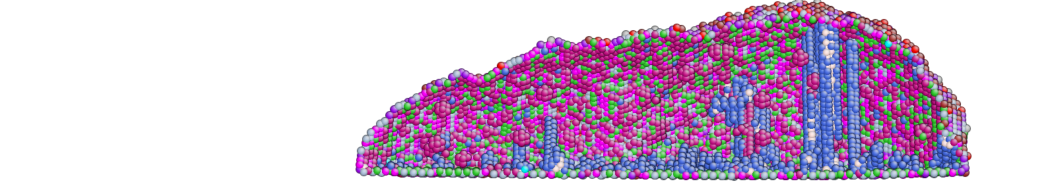
\includegraphics[width=0.99\linewidth]{Chap4/plots/Picture9c.pdf}}\label{Chap:Ag/ZnO:fig:9c}
\caption[Common neighbor analysis and centro-symmetry analysis for Ag thin film quality on rectangular substrates.]{\ac{CNA} and centro-symmetry analysis for Ag thin film quality on rectangular substrates. (a) \ac{CNA} for Ag thin film deposited on substrate with bond length of 2.9$\angstrom$. (b) common neighbor analysis for Ag thin film deposited on substrate with bond length of 3.3$\angstrom$. (c) centro-symmetry analysis for Ag thin film deposited on substrate with bond length of 3.3$\angstrom$. Lines formed by blue atoms indicating misfit dislocations.}
  \label{Chap:Ag/ZnO:fig9}
\end{figure}
\endgroup

\newpage
\begingroup
\begin{figure}[!ht]
  \centering
  \subfigure[]{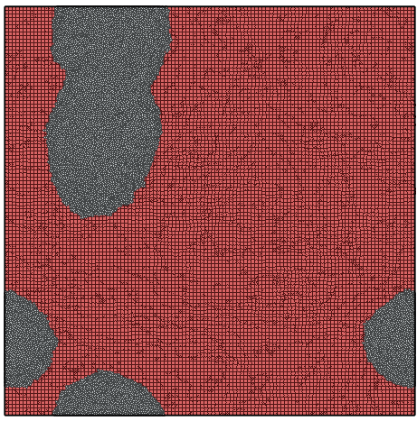
\includegraphics[width=0.35\linewidth]{Chap4/plots/Picture10a.pdf}}\label{Chap:Ag/ZnO:fig:10a}
  \subfigure[]{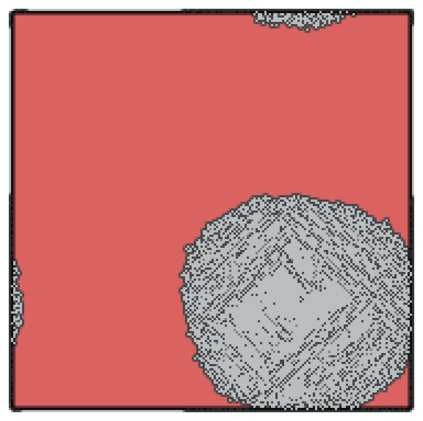
\includegraphics[width=0.35\linewidth]{Chap4/plots/Picture10b.pdf}}\label{Chap:Ag/ZnO:fig:10b}
  \\
  \subfigure[]{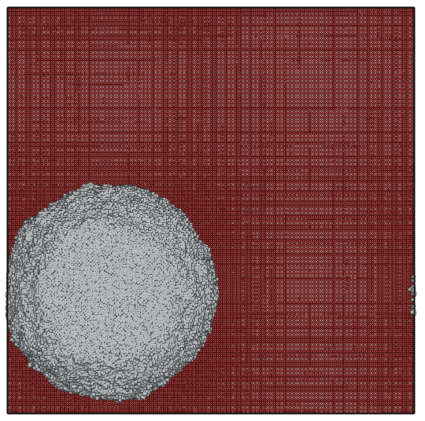
\includegraphics[width=0.35\linewidth]{Chap4/plots/Picture10c.pdf}}\label{Chap:Ag/ZnO:fig:10c}
  \subfigure[]{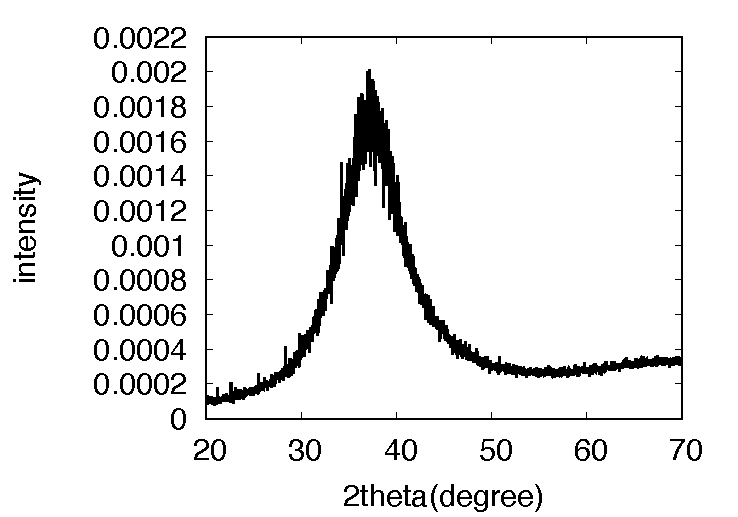
\includegraphics[width=0.45\linewidth]{Chap4/plots/Picture10d.pdf}}\label{Chap:Ag/ZnO:fig:10d}
  \\
  \subfigure[]{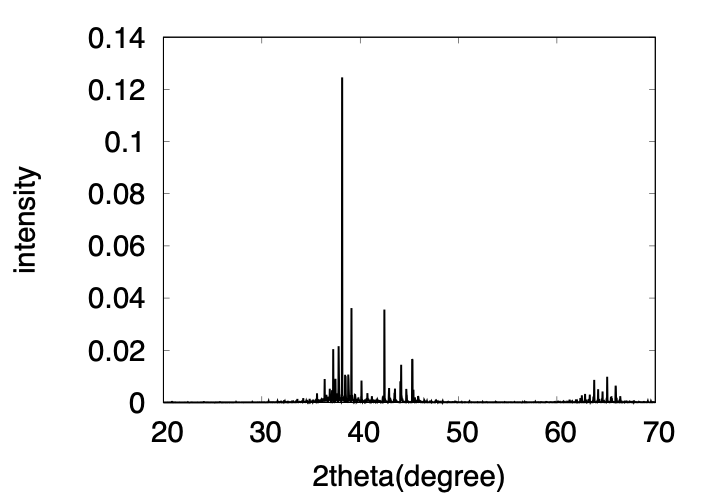
\includegraphics[width=0.45\linewidth]{Chap4/plots/Picture10e.png}}\label{Chap:Ag/ZnO:fig:10e}
  \subfigure[]{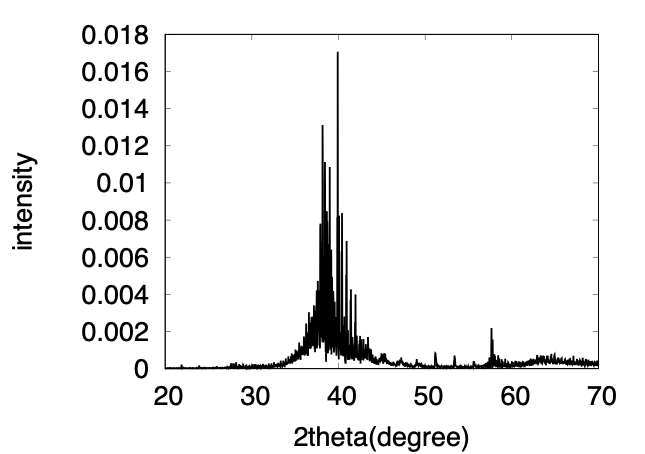
\includegraphics[width=0.45\linewidth]{Chap4/plots/Picture10f.png}}\label{Chap:Ag/ZnO:fig:10f}

\caption[GCMC simulation results of Ag thin film morphology on square substrates.]{Top-view of \ac{GCMC} simulated Ag thin film morphology on square substrates with bond length of (a) 2.3$\angstrom$, (b) 2.9$\angstrom$, and (c) 3.3$\angstrom$. (d), (e), and (f) are corresponding simulated \ac{XRD} results of three Ag thin film  deposited on substrates with previously mentioned bond length.}
  \label{Chap:Ag/ZnO:fig10-1}
\end{figure}
\endgroup


\begingroup
\begin{figure}[!ht]
  \centering
  \subfigure[]{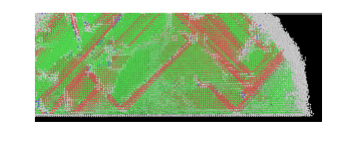
\includegraphics[width=0.65\linewidth]{Chap4/plots/Picture10g.png}}\label{Chap:Ag/ZnO:fig:10g}
  \subfigure[]{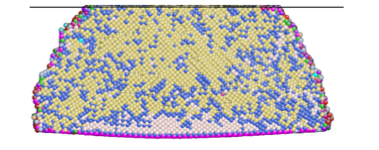
\includegraphics[width=0.65\linewidth]{Chap4/plots/Picture10h.png}}\label{Chap:Ag/ZnO:fig:10h}
\caption[Side-view of \ac{GCMC} simulated Ag thin film morphology on square substrates.]{Side-view of \ac{GCMC} simulated Ag thin film morphology on square substrates. (a) \ac{CNA} for Ag thin film deposited on substrate with bond length of 2.9$\angstrom$. (b) coordination number of Ag thin film deposited on substrate with bond length of 3.3$\angstrom$. Yellow, blue and pink color are atoms with coordination numbers of 12, 11, 14 (second nearest neighbors included).}
  \label{Chap:Ag/ZnO:fig10-3}
\end{figure}
\endgroup

Next, we investigated Ag thin film morphology and qualities on rectangular-shaped substrates. As shown in Fig. \ref{Chap:Ag/ZnO:fig8}, only Ag bond length substrate yields a continuous Ag thin film. Both higher and lower bond length substrates grow 3-D islands. Besides, From \ac{XRD} results, Ag grown on substrates with lower bond length are amorphous, which will greatly affect Ag thin film quality. Strong \ac{HCP} peaks are observed with a substrate of higher bond length. In Fig. \ref{Chap:Ag/ZnO:fig:9a} and \ref{Chap:Ag/ZnO:fig:9b}, \ac{CNA} analysis is conducted for Ag thin film deposited on substrate with bond length of 2.9$\angstrom$ and 3.3$\angstrom$. The majority of the thin film is \ac{HCP} phase with a small amount of vertically layered defects. Besides, centrosymmetric analysis is conducted for 3.3$\angstrom$ substrate, as shown in Fig. \ref{Chap:Ag/ZnO:fig:9c}. Vertical-oriented misfit dislocations are generated to release strain energy from lattice mismatch. Based on the above observation, Ag thin film quality on rectangular lattice substrates is sensitive to substrate lattice constant change. A similar conclusion also applies to square lattice substrates. As shown in Fig. \ref{Chap:Ag/ZnO:fig:10d}, amorphous phase comes out with decreasing lattice constant. When the substrate lattice constant increases, several nm of \ac{BCC} layers appear at the interface. 

\newpage
\begingroup
\begin{figure}[!ht]
  \centering
  \subfigure[]{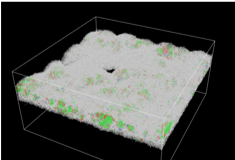
\includegraphics[width=0.5\linewidth]{Chap4/plots/Picture11a.png}}\label{Chap:Ag/ZnO:fig:11a}
  \subfigure[]{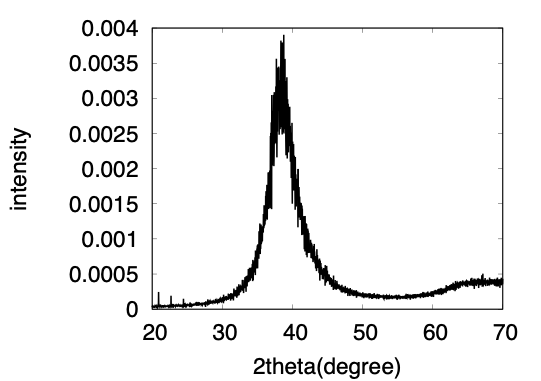
\includegraphics[width=0.65\linewidth]{Chap4/plots/Picture11b.png}}\label{Chap:Ag/ZnO:fig:11b}
\caption[CNA and Simulated XRD results of Ag thin film morphology on an amorphous substrate.]{(a) \ac{CNA} and (b) Simulated \ac{XRD} results of Ag thin film morphology on an amorphous substrate.}
\label{Chap:Ag/ZnO:fig11}
\end{figure}
\endgroup

At last, Ag thin film is also deposited on an amorphous substrate during \ac{GCMC} simulation. As shown in Fig. \ref{Chap:Ag/ZnO:fig:11a}, the thin film is more continuous compared to other ordered lattice substrate structures, because of amorphous substrates containing more surface defects acting as a trap site for Ag adsorbates. However, the quality of Ag thin film is not desirable for industry use, as the thin film shows an amorphous structure from the \ac{XRD}.